\documentclass[a4paper,10pt]{article}
\usepackage{beamerarticle}
\setjobnamebeamerversion{overview-b}

\usepackage{fullpage}

\usepackage[backend=biber,url=false,style=alphabetic]{biblatex}
\addbibresource{os.bib}

\usepackage{hyperref}
\usepackage[textsize=footnotesize]{todonotes}
\addtolength{\oddsidemargin}{-15pt}
\addtolength{\marginparsep}{5pt}
% \setlength{\marginparwidth}{1.2in}
% \let\oldmarginpar\marginpar
% \renewcommand\marginpar[1]{\-\oldmarginpar[\raggedleft\footnotesize #1]%
% {\raggedright\footnotesize #1}}
\newcommand{\Marginpar}[1]{\marginpar{\raggedright{\footnotesize \emph{#1}}}}

% http://tex.stackexchange.com/q/25259/86
% for *notes*
\defbeamertemplate<article>{frame begin}{lined}{
  \par\noindent\rule{\textwidth}{2pt}\par}
\defbeamertemplate<article>{frame end}{lined}{
  \par\vspace{1em}\noindent\rule{.1\textwidth}{.3pt}
  \raisebox{-3pt}{{\large \Info}}
  \rule{.1618\textwidth}{.3pt}\par\vspace{.5em}}

\setbeamertemplate{frame begin}[lined]
\setbeamertemplate{frame end}[lined]

%\documentclass[10pt,xcolor=svgnames,ignorenonframetext,hyperref={xetex,colorlinks,linkcolor=blue},compress]{beamer}

\usepackage{pgfpages}

\usepackage{latexsym,pifont,units,amsmath,amsfonts,amssymb,marvosym}
\usepackage{xltxtra} %fontspec,xunicode are loaded here.
\defaultfontfeatures{Mapping=tex-text}
\setsansfont{DejaVu Sans}
\setmainfont{DejaVu Serif}

% \usepackage{graphicx} % beamer loads graphicx already.
\graphicspath{{./figs/}{../figs/}{./}{../}} %note that the trailing “/” is required

\usepackage{tikz}
\usetikzlibrary{arrows,decorations.pathmorphing,backgrounds,positioning,fit}

\usepackage{multicol,varwidth}

\newcommand{\cfbox}[2]{%
  \colorlet{currentcolor}{.}%
  {\color{#1}\fbox{\color{currentcolor}#2}}%
}

\newcommand{\code}[1]{\texttt{\textcolor{violet}{#1}}}

\mode<beamer>{
  \usetheme{default}
  \usecolortheme{sidebartab}
  \usefonttheme{serif}
  \setbeamertemplate{footline}[frame number]
  \setbeamertemplate{navigation symbols}{}
  \usenavigationsymbolstemplate{}
  \setbeamertemplate{blocks}[rounded][shadow=true]
  \setbeamercolor{structure}{fg=Green}
  \setbeamercolor{block title}{fg=Green}
}

\begin{document}

\mode<article>{ \title{Linux Kernel Introduction} \author{Wang
    Xiaolin\\wx672ster@gmail.com}
  \maketitle
  \tableofcontents
  \printbibliography
  \clearpage
}

\begin{frame}<beamer> \title{Linux Kernel Introduction} \author{Wang Xiaolin} \titlepage
  \vfill \tiny{ \ding{41} wx672ster@gmail.com
    % \ding{37} 13577067397
  }
\end{frame}

\section{Basic Operating System Concepts}
\label{sec:basic-oper-syst}

\begin{frame}{Basic Operating System Concepts}
  \begin{exampleblock}{Two main objectives of an OS:}
    \begin{itemize}
    \item Interact with the hardware components
    \item Provide an execution environment to the applications
    \end{itemize}
  \end{exampleblock}
  \begin{exampleblock}{Why?}
    \begin{description}
    \item[Unix] hides all low-level details from applications
      \begin{itemize}
      \item[] \emph{User mode vs. Kernel mode}
      \end{itemize}
    \item[MS-DOS] allows user programs to directly play with the hardware components
    \end{description}
  \end{exampleblock}
\end{frame}

\begin{description}
\item[UNIX] The original elegant design of the Unix system, along with the years of
  innovation and evolutionary improvement that followed, have made Unix a powerful,
  robust, and stable operating system. A handful of characteristics of Unix are
  responsible for its resilience.\cite{love2010linux}
  \begin{itemize}
  \item First, Unix is simple: Whereas some operating systems implement thousands of
    system calls and have unclear design goals, Unix systems typically implement only
    hundreds of system calls and have a very clear design.
  \item Next, in Unix, \emph{everything is a file}. This simplifies the manipulation of
    data and devices into a set of simple system calls: \code{open()}, \code{read()},
    \code{write()}, \code{ioctl()}, and \code{close()}.
  \item In addition, the Unix kernel and related system utilities are written in C --- a
    property that gives Unix its amazing portability and accessibility to a wide range of
    developers.
  \item Next, Unix has fast process creation time and the unique \code{fork()} system
    call. This encourages strongly partitioned systems without gargantuan multi-threaded
    monstrosities.
  \item Finally, Unix provides simple yet robust interprocess communication (IPC)
    primitives that, when coupled with the fast process creation time, allow for the
    creation of simple utilities that do one thing and do it well, and that can be strung
    together to accomplish more complicated tasks.
  \end{itemize}
\end{description}

\begin{frame}
  \begin{exampleblock}{Typical Components of a Kernel}
    \begin{description}
    \item[Interrupt handlers:] to service interrupt requests
    \item[Scheduler:] to share processor time among multiple processes
    \item[Memory management system:] to manage process address spaces
    \item[System services:] Networking, IPC...
    \end{description}
  \end{exampleblock}
\end{frame}

\begin{frame}{Kernel And Processes}
  \begin{exampleblock}{Kernel space}
    \begin{itemize}
    \item a protected memory space
    \item full access to the hardware
    \end{itemize}
    When executing the kernel, the system is in kernel-space executing in \emph{kernel
      mode}.
  \end{exampleblock}
  \begin{exampleblock}{User Space}
    \begin{itemize}
    \item Can only see a subset of available resources
    \item unable to perform certain system functions, nor directly access hardware
    \end{itemize}
    Normal user execution in user-space executing in \emph{user mode}.
  \end{exampleblock}
  $$\text{user mode} \xrightarrow{system\ calls} \text{kernel mode}$$
\end{frame}

\begin{frame}
  \begin{center}
    \mode<beamer>{
      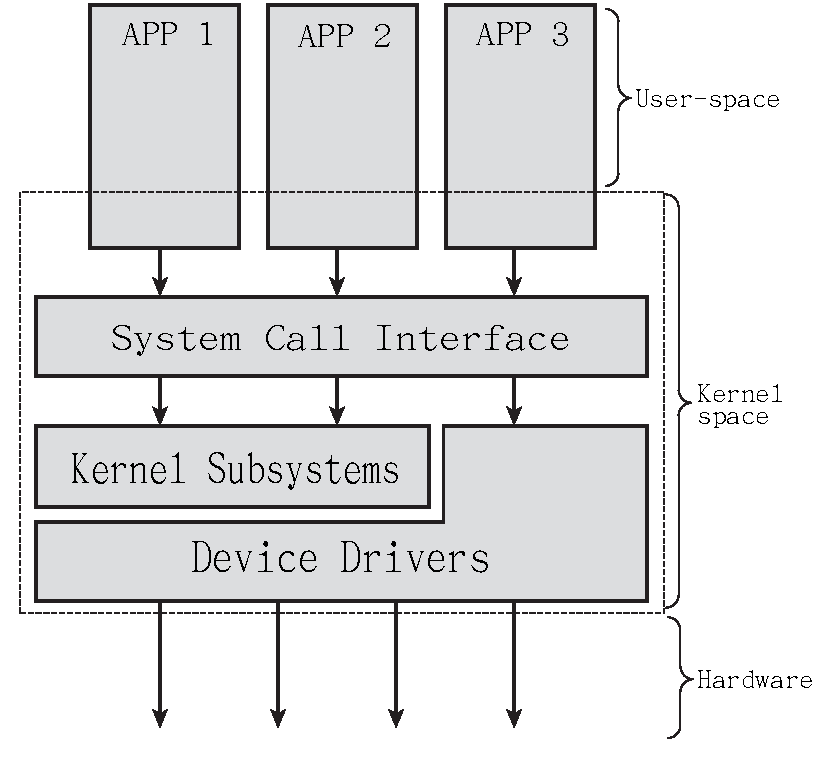
\includegraphics[width=.8\textwidth]{overview}
    } \mode<article>{
      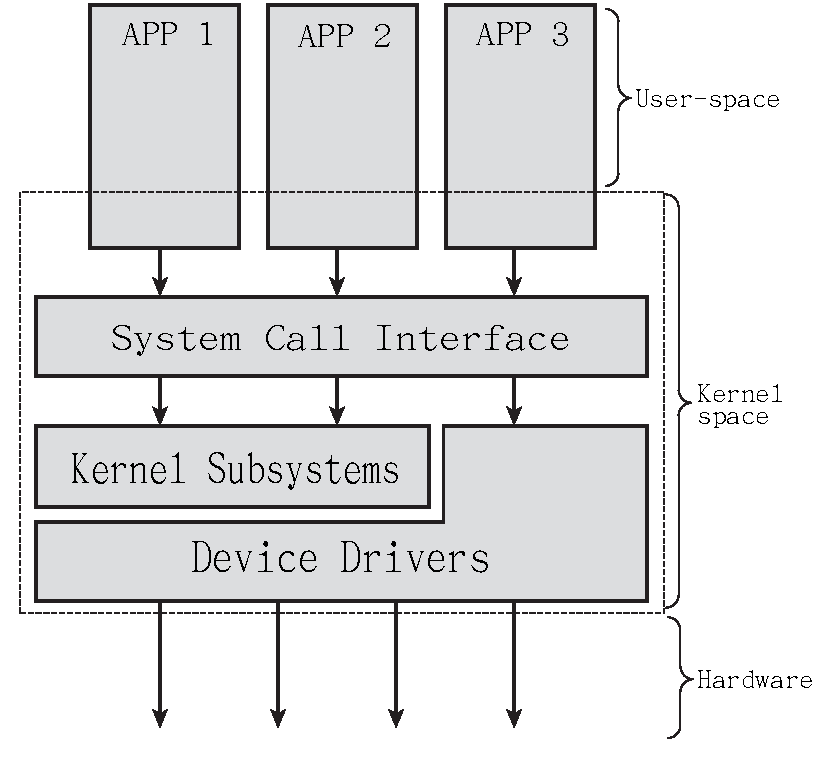
\includegraphics[width=.6\textwidth]{overview}
    }
  \end{center}
\end{frame}

\begin{description}
\item[C library and system calls] An application typically calls functions in a library,
  for example, the \emph{C library}, that in turn rely on the system call interface to
  instruct the kernel to carry out tasks on their behalf. Some library calls provide many
  features not found in the system call, and thus, calling into the kernel is just one
  step in an otherwise large function. For example, consider the familiar \code{printf()}
  function. It provides formatting and buffering of the data and only eventually calls
  \code{write()} system call to write the data to the console. Conversely, some library
  calls have a one-to-one relationship with the kernel. For example, the \code{open()}
  library function does nothing except call the \code{open()} system call. Still other C
  library functions, such as \code{strcpy()}, should (you hope) make no use of the kernel
  at all. When an application executes a system call, it is said that the \emph{kernel is
    executing on behalf of the application}. Furthermore, the application is said to be
  \emph{executing a system call in kernel-space}, and the kernel is running in
  \emph{process context}. This relationship that applications \emph{call into} the kernel
  via the system call interfaceis the fundamental manner in which applications get work
  done.\cite{love2010linux}
\end{description}

\begin{frame}{Kernel And Hardware}
  \begin{exampleblock}{Interrupts}
    Whenever hardware wants to communicate with the system, it issues an interrupt that
    asynchronously interrupts the kernel.
    \begin{description}
    \item[Interrupt vector]
    \item[Interrupt handlers]
    \end{description}
  \end{exampleblock}
\end{frame}

\begin{description}
\item[Interrupts] The kernel also manages the system's hardware. Nearly all architectures,
  including all systems that Linux supports, provide the concept of
  \emph{interrupts}. When hardware wants to communicate with the system, it issues an
  interrupt that asynchronously interrupts the kernel. Interrupts are identified by a
  number. The kernel uses the number to execute a specific \emph{interrupt handler} to
  process and respond to the interrupt. For example, as you type, the keyboard controller
  issues an interrupt to let the system know that there is new data in the keyboard
  buffer. The kernel notes the interrupt number being issued and executes the correct
  interrupt handler. The interrupt handler processes the keyboard data and lets the
  keyboard controller know it is ready for more data. To provide synchronization, the
  kernel can usually disable interrupts, either all interrupts or just one specific
  interrupt number. In many operating systems, including Linux, the interrupt handlers do
  not run in a process context. Instead, they run in a special \emph{interrupt context}
  that is not associated with any process. This special context exists solely to let an
  interrupt handler quickly respond to an interrupt, and then exit.\cite{love2010linux}

  These contexts represent the breadth of the kernel's activities. In fact, in Linux, we
  can generalize that each processor is doing one of three things at any given moment:
  \begin{itemize}
  \item In kernel-space, in process context, executing on behalf of a specific process
  \item In kernel-space, in interrupt context, not associated with a process, handling an
    interrupt
  \item In user-space, executing user code in a process
  \end{itemize}
  This list is inclusive. Even corner cases fit into one of these three activities: For
  example, when idle, it turns out that the kernel is executing an \emph{idle process} in
  process context in the kernel.
\end{description}

\begin{frame}{Kernel Architecture}%{Basic Operating System Concepts}
  \begin{exampleblock}{Monolithic kernels}
    Simplicity and performance
    \begin{itemize}
    \item exist on disk as single static binaries
    \item All kernel services run in the kernel address space
    \item Communication within the kernel is trivial
    \end{itemize}
    Most Unix systems are monolithic in design.
  \end{exampleblock}
\end{frame}

\begin{frame}
  \begin{exampleblock}{Microkernels}
    \begin{itemize}
    \item are not implemented as single large processes
    \item break the kernel into separate processes (\emph{servers}).
      \begin{multicols}{2}
        \begin{itemize}
        \item in the microkernel
          \begin{itemize}
          \item a few synchronization primitives
          \item a simple scheduler
          \item an IPC mechanism
          \end{itemize}
        \item top of the microkernel
          \begin{itemize}
          \item memory allocators
          \item device drivers
          \item system call handlers
          \end{itemize}
        \end{itemize}
      \end{multicols}
    \end{itemize}
  \end{exampleblock}
\end{frame}

\begin{frame}
  \begin{exampleblock}{Advantages of microkernel OS}
    \begin{itemize}
    \item modularized design
    \item easily ported to other architectures
    \item make better use of RAM
    \end{itemize}
  \end{exampleblock}
  \begin{exampleblock}{Performance Overhead}
    \begin{itemize}
    \item Communication via \emph{message passing}
    \item Context switch (kernel-space $\Leftrightarrow$ user-space)
      \begin{itemize}
      \item Windows NT and Mac OS X keep all servers in kernel-space. (defeating the
        primary purpose of microkernel designs)
      \end{itemize}
    \end{itemize}
  \end{exampleblock}
  \begin{itemize}
  \item Microkernel OSes are generally slower than monolithic ones.
  \item Academic research on OS is oriented toward microkernels.
  \end{itemize}
\end{frame}

\begin{description}
\item[Monolithic Kernel Versus Microkernel Designs] Operating kernels can be divided into
  two main design camps: the monolithic kernel and the microkernel. (A third camp,
  exokernel, is found primarily in research systems but is gaining ground in real-world
  use.)

  Monolithic kernels involve the simpler design of the two, and all kernels were designed
  in this manner until the 1980s. Monolithic kernels are implemented entirely as single
  large processes running entirely in a single address space. Consequently, such kernels
  typically exist on disk as single static binaries. All kernel services exist and execute
  in the large kernel address space. Communication within the kernel is trivial because
  everything runs in kernel mode in the same address space: The kernel can invoke
  functions directly, as a user-space application might. Proponents of this model cite the
  simplicity and performance of the monolithic approach. Most Unix systems are monolithic
  in design.

  Microkernels, on the other hand, are not implemented as single large processes. Instead,
  the functionality of the kernel is broken down into separate processes, usually called
  servers. Idealistically, only the servers \emph{absolutely} requiring such capabilities
  run in a privileged execution mode. The rest of the servers run in user-space. All the
  servers, though, are kept separate and run in different address spaces. Therefore,
  direct function invocation as in monolithic kernels is not possible. Instead,
  communication in microkernels is handled via \emph{message passing}: An interprocess
  communication (IPC) mechanism is built into the system, and the various servers
  communicate and invoke "services" from each other by sending messages over the IPC
  mechanism. The separation of the various servers prevents a failure in one server from
  bringing down another.

  Likewise, the modularity of the system allows one server to be swapped out for
  another. Because the IPC mechanism involves quite a bit more overhead than a trivial
  function call, however, and because a context switch from kernel-space to user-space or
  vice versa may be involved, message passing includes a latency and throughput hit not
  seen on monolithic kernels with simple function invocation. Consequently, all practical
  microkernel-based systems now place most or all the servers in kernel-space, to remove
  the overhead of frequent context switches and potentially allow for direct function
  invocation. The Windows NT kernel and Mach (on which part of Mac OS X is based) are
  examples of microkernels. Neither Windows NT nor Mac OS X run any microkernel servers in
  user-space in their latest versions, defeating the primary purpose of microkernel
  designs altogether.

  Linux is a monolithic kernel, that is, the Linux kernel executes in a single address
  space entirely in kernel mode. Linux, however, borrows much of the good from
  microkernels: Linux boasts a modular design with kernel preemption, support for kernel
  threads, and the capability to dynamically load separate binaries (kernel modules) into
  the kernel. Conversely, Linux has none of the performance-sapping features that curse
  microkernel designs: Everything runs in kernel mode, with direct function invocation,
  not message passing, the method of communication. Yet Linux is modular, threaded, and
  the kernel itself is schedulable. Pragmatism wins again.\cite{love2010linux}
\end{description}


% \section{An Overview of the Unix Filesystem}
% \label{sec:an-overview-unix}

% \begin{frame}{An Overview of the Unix Filesystem}
%   \begin{multicols}{2}
%     \begin{itemize}
%     \item directory tree
%     \item hard and soft links
%     \item file types
%     \item file descriptor and inode
%     \item access rights and file mode
%     \end{itemize}
%   \end{multicols}
%   \begin{exampleblock}{file-handling syscalls}
%     \begin{center}
%       \begin{tabular}{rcl}
%         \code{fd}&\code{=}&\code{open(path, flag, mode);}\\
%         \code{newoffset}&\code{=}&\code{lseek(fd, offset, whence);}\\
%         \code{nread}&\code{=}&\code{read(fd, buf, count);}\\
%         \code{nwrite}&\code{=}&\code{write(fd, buf, count);}\\
%         \code{status}&\code{=}&\code{close(fd);}\\
%         \code{status}&\code{=}&\code{rename(oldpath, newpath);}\\
%         \code{status}&\code{=}&\code{unlink(pathname);}
%       \end{tabular}
%     \end{center}
%   \end{exampleblock}
% \end{frame}

\section{Linux Versus Other Unix-Like Kernels}
\label{sec:linux-versus-other}

\begin{frame}
  \begin{exampleblock}{Linux is a monolithic kernel with modular design}
    \begin{description}
    \item[Modularized approach] --- makes it easy to develop new modules
    \item[Platform independence] --- if standards compliant
    \item[Frugal main memory usage] --- run time (un)loadable
    \item[No performance penalty] --- no explicit message passing is required
    \end{description}
  \end{exampleblock}
\end{frame}

\begin{frame}{Linux}
  \begin{exampleblock}{A newcomer in the family of Unix-like OSes}
    \begin{center}
      \begin{tabular}{lll}
        AT\&T Unix SVR4&UCB 4.4BSD& DEC Digital Unix\\
        IBM AIX& HP HP-UX& Sun Solaris\\
        Apple Mac OS X& FreeBSD& NetBSD\\
        OpenBSD& Linux&
      \end{tabular}
    \end{center}
    \begin{itemize}
    \item Linus Torvalds, 1991
    \item A true Unix kernel
    \item available on many architectures
      \begin{itemize}
      \item \code{ls /usr/src/linux/arch/}
      \end{itemize}
    \item GPL, non-commercial
    \end{itemize}
  \end{exampleblock}
\end{frame}

\begin{frame}%
  \begin{exampleblock}{Linux Versus Other Unix-Like Kernels}
    \begin{itemize}
    \item share fundamental design ideas and features
    \item from 2.6, Linux kernels are POSIX-compliant
      \begin{itemize}
      \item Unix programs can be compiled and executed on Linux
      \end{itemize}
    \item Linux includes all the features of a modern Unix
      \begin{itemize}
      \item VM, VFS, LWP, SVR4 IPC, signals, SMP support ...
      \end{itemize}
    \end{itemize}
  \end{exampleblock}
\end{frame}

\begin{frame}
  \begin{exampleblock}{Linux Kernel Features}
    \begin{itemize}
    \item Monolithic kernel
    \item loadable modules support
    \item Kernel threading
    \item Multithreaded application support
    \item Preemptive kernel
    \item Multiprocessor support
    \item File systems
    \end{itemize}
  \end{exampleblock}
\end{frame}

\begin{frame}
  \begin{exampleblock}{Advantages Over Its Commercial Competitors}
    \begin{itemize}
    \item cost-free
    \item fully customizable in all its components
    \item runs on low-end, inexpensive hardware platforms
    \item performance
    \item developers are excellent programmers
    \item kernel can be very small and compact
    \item highly compatible with many common operating systems
      \begin{itemize}
      \item filesystems, network interfaces, wine ...
      \end{itemize}
    \item well supported
    \end{itemize}
  \end{exampleblock}
\end{frame}

\begin{frame}{Linux Versions}
  \begin{center}
    \mode<beamer>{
      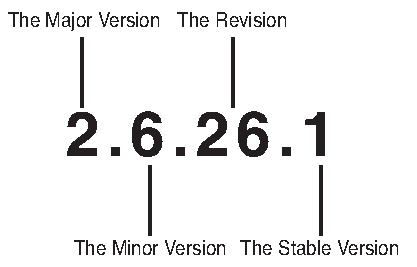
\includegraphics[width=.7\textwidth]{version}
    } \mode<article>{
      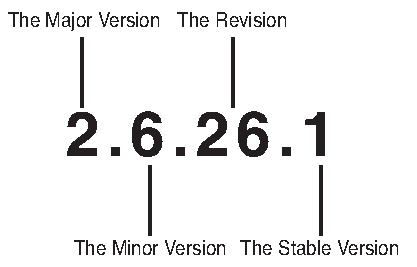
\includegraphics[width=.4\textwidth]{version}
    }
  \end{center}
\end{frame}

\section{An Overview of Unix Kernels}
\label{sec:an-overview-unix-1}

\subsection{The Process/Kernel Model}
\label{sec:processkernel-model}

\begin{frame}{The Unix Process/Kernel Model}%{An Overview of Unix Kernels}
  \begin{exampleblock}{User Mode vs. Kernel Mode}
    \begin{itemize}
    \item Processes can run in either user mode or kernel mode
    \item The kernel itself is not a process but a process manager
    \end{itemize}
  \end{exampleblock}
  $$\text{processes} \xrightarrow{system\ calls} \text{process manager}$$
\end{frame}

\begin{frame}
  \begin{exampleblock}{Kernel routines can be activated in several ways}
    \begin{center}
      \mode<beamer>{
        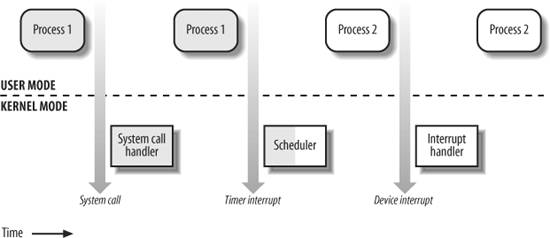
\includegraphics[width=.8\textwidth]{understandlk_0102}
      } \mode<article>{
        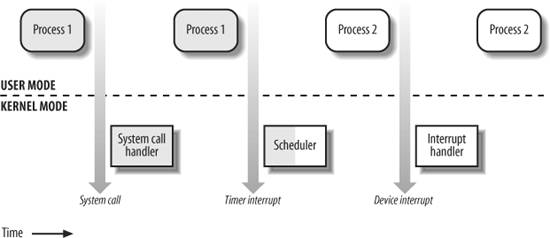
\includegraphics[width=.5\textwidth]{understandlk_0102}
      }
    \end{center}
  \end{exampleblock}
\end{frame}

\begin{frame}
  \begin{exampleblock}{Unix Kernel Threads}
    \begin{itemize}
    \item run in Kernel Mode in the kernel address space
    \item no interact with users
    \item created during system startup and remain alive until the system is
      shut down
    \end{itemize}
  \end{exampleblock}
\end{frame}

\subsection{Process Implementation}
\label{sec:proc-impl}

\begin{frame}
  \begin{exampleblock}{Process Implementation}
    \begin{itemize}
    \item Each process is represented by a \emph{process descriptor (PCB)}
    \item Upon a process switch, the kernel
      \begin{itemize}
      \item saves the current contents of several registers in the PCB
      \item uses the proper PCB fields to load the CPU registers
      \end{itemize}
    \end{itemize}
  \end{exampleblock}
  \begin{exampleblock}{Registers}
    \begin{itemize}
    \item The program counter (PC) and stack pointer (SP) registers
    \item The general purpose registers
    \item The floating point registers
    \item The processor control registers (Processor Status Word) containing information
      about the CPU state
    \item The memory management registers used to keep track of the RAM accessed by the
      process
    \end{itemize}
  \end{exampleblock}
\end{frame}

\subsection{Reentrant Kernels}
\label{sec:reentrant-kernels}

\begin{frame}{Reentrant Kernels}
  \begin{description}
  \item[Reentrant Kernels] several processes may be executing in Kernel Mode at the same
    time
    \begin{itemize}
    \item[i.e.] several processes can wait in kernel mode
    \end{itemize}
  \item[Kernel control path] denotes the sequence of instructions executed by the kernel
    to handle a system call, an exception, or an interrupt.
  \end{description}
  \begin{exampleblock}{Interleaving of kernel control paths}
    \begin{center}
      \mode<article>{
        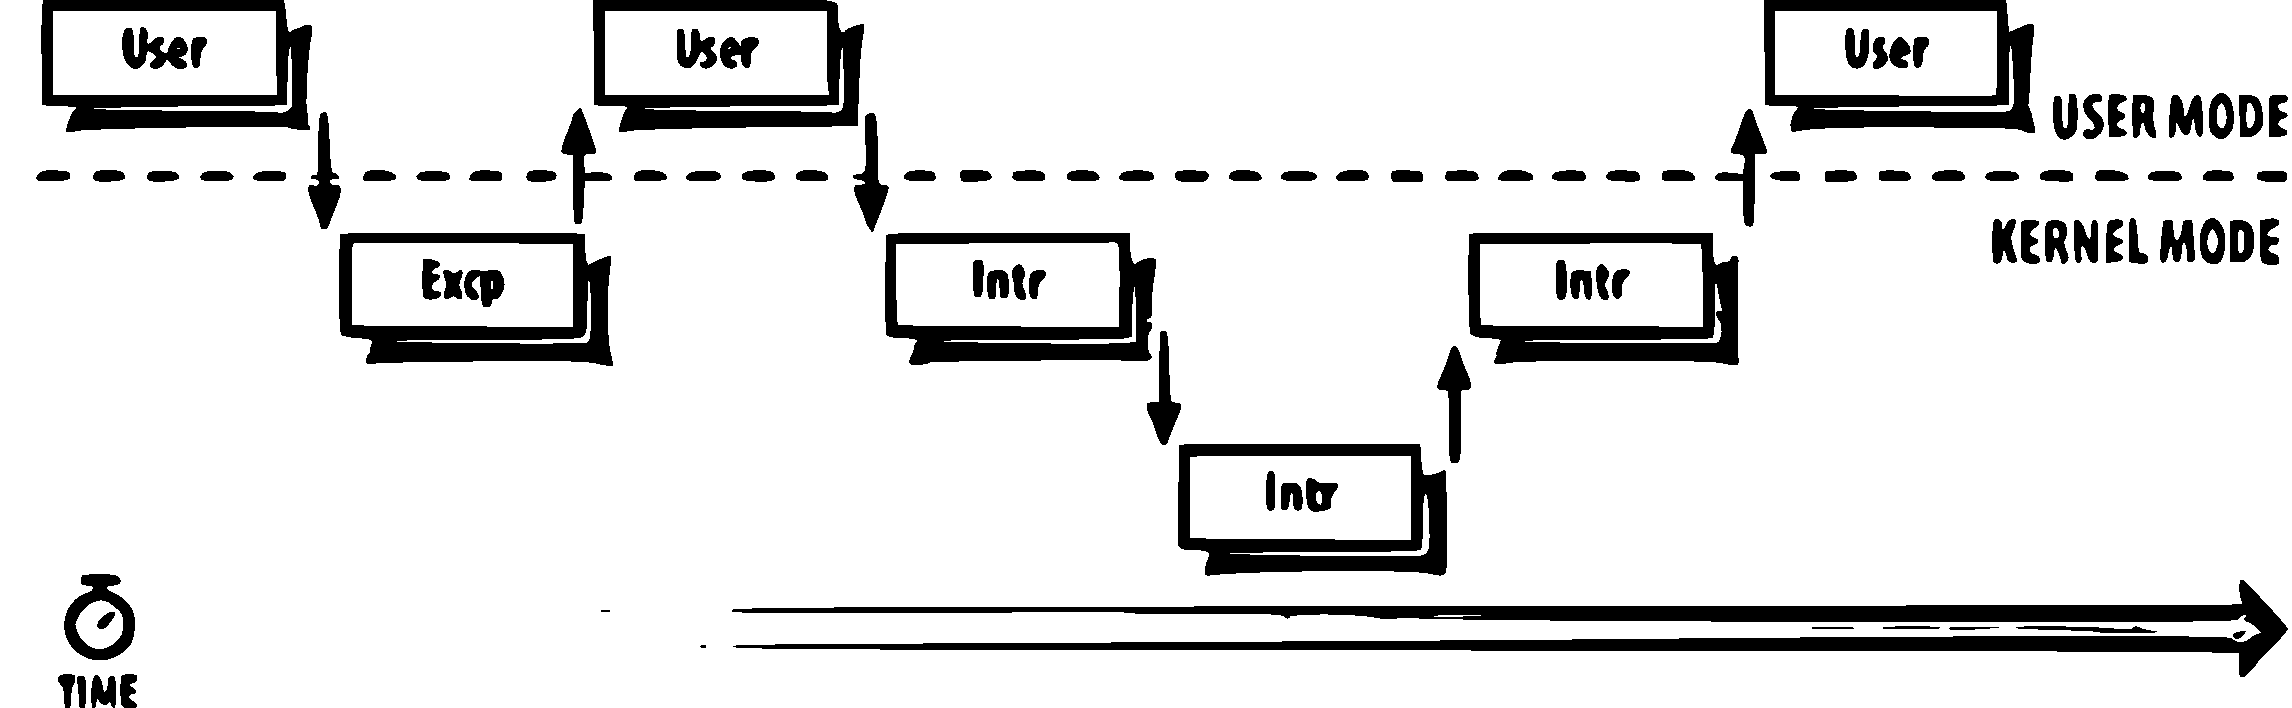
\includegraphics[width=.5\textwidth]{understandlk_0103}
      } \mode<beamer>{
        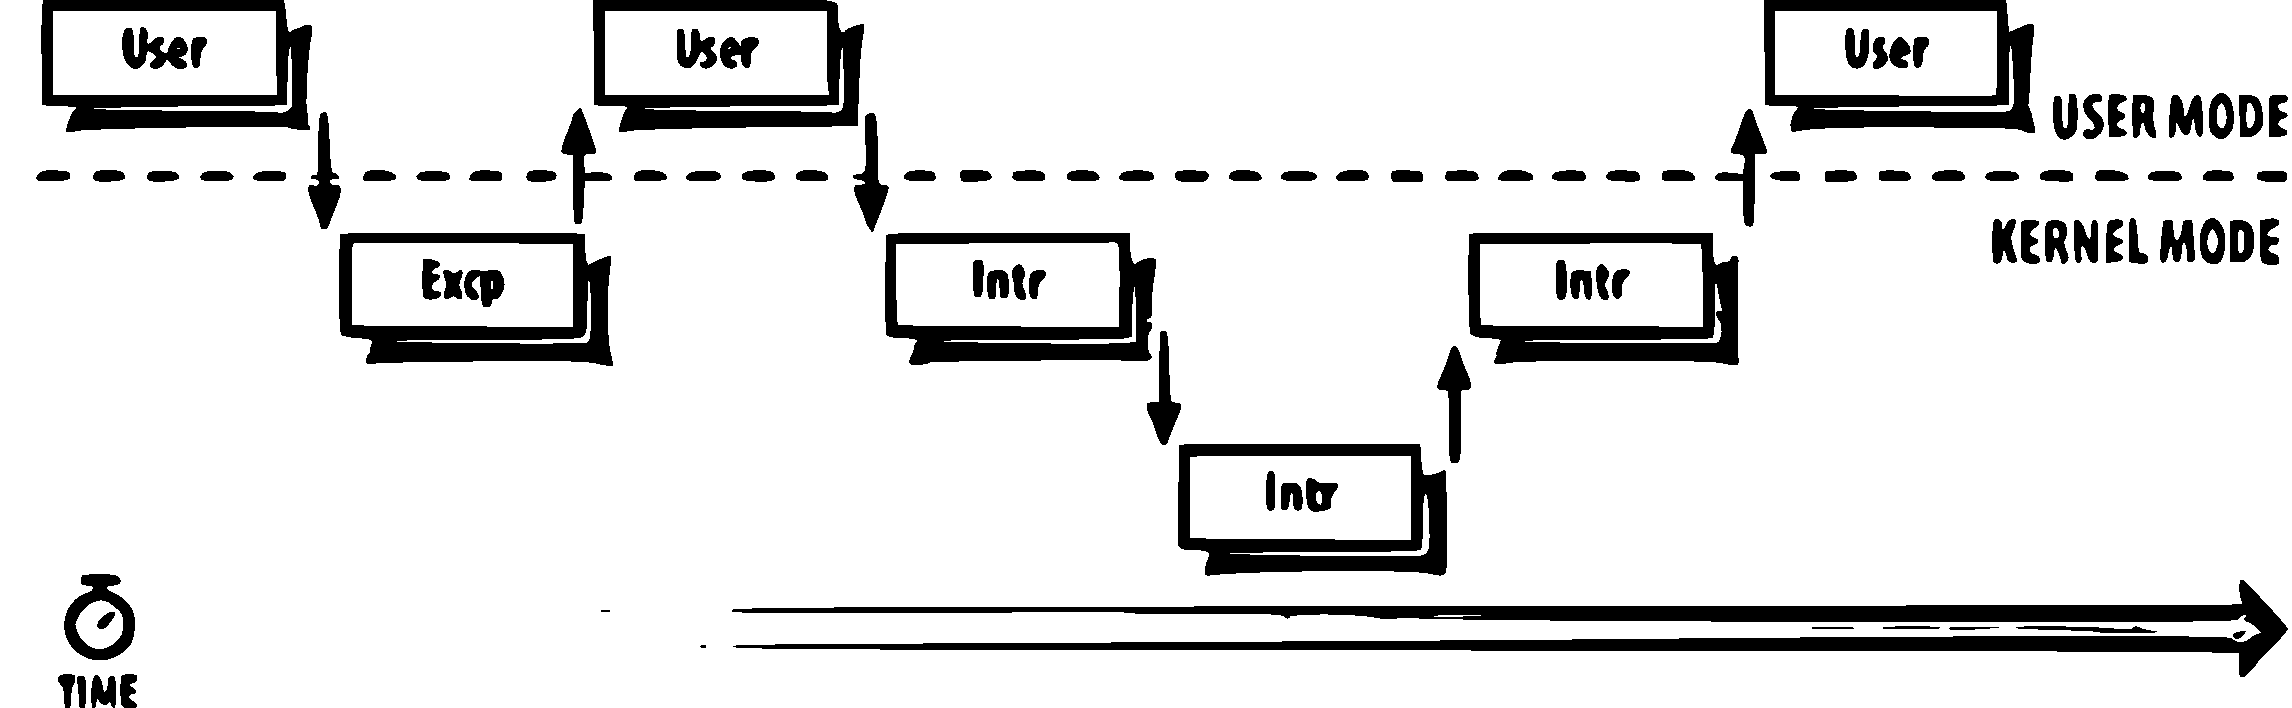
\includegraphics[width=\textwidth]{understandlk_0103}
      }
    \end{center}
  \end{exampleblock}
\end{frame}

\begin{description}
\item[Re-entrant functions] It's easier to remember when you understand what the term
  means.

  The term "re-entrant" means that it is safe to "re-enter" the function while it is
  already executed, typically in a concurrent environment.

  In other words, when two tasks can execute the function at the same time without
  interfering with each other, then the function is re-entrant. A function is not
  re-entrant when the execution by one task has an impact on the influence of another
  task. This typically is the case when a global state or data is used. A function that
  uses only local variables and arguments is typically
  re-entrant. [\href{http://stackoverflow.com/questions/261311/what-is-the-difference-between-re-entrant-function-and-recursive-function-in-c}{Stackoverflow}]
\item[About kernel control path] (Sec 1.6.3 in \cite{bovet2005understanding}) In the
  simplest case, the CPU executes a kernel control path sequentially from the first
  instruction to the last. When one of the following events occurs, however, the CPU
  interleaves the kernel control paths :
  \begin{itemize}
  \item[case 1] A process executing in User Mode invokes a system call, and the corresponding
    kernel control path verifies that the request cannot be satisfied immediately; it then
    invokes the scheduler to select a new process to run. As a result, a process switch
    occurs. The first kernel control path is left unfinished, and the CPU resumes the
    execution of some other kernel control path. In this case, the two control paths are
    executed on behalf of two different processes.
  \item[case 2] The CPU detects an exception, for example, access to a page not present in
    RAM, while running a kernel control path. The first control path is suspended, and the
    CPU starts the execution of a suitable procedure. In our example, this type of
    procedure can allocate a new page for the process and read its contents from
    disk. When the procedure terminates, the first control path can be resumed. In this
    case, the two control paths are executed on behalf of the same process.
  \item[case 3] A hardware interrupt occurs while the CPU is running a kernel control path with
    the interrupts enabled. The first kernel control path is left unfinished, and the CPU
    starts processing another kernel control path to handle the interrupt. The first
    kernel control path resumes when the interrupt handler terminates. In this case, the
    two kernel control paths run in the execution context of the same process, and the
    total system CPU time is accounted to it. However, the interrupt handler doesn't
    necessarily operate on behalf of the process.
  \item[case 4] An interrupt occurs while the CPU is running with kernel preemption
    enabled, and a higher priority process is runnable. In this case, the first kernel
    control path is left unfinished, and the CPU resumes executing another kernel control
    path on behalf of the higher priority process. This occurs only if the kernel has been
    compiled with kernel preemption support.
  \item
    \href{http://stackoverflow.com/questions/8453294/userspace-process-preempts-kernel-thread}{stackoverflow:
      User-space process preempts kernel thread?}
  \end{itemize}
\end{description}

\subsection{Process Address Space}
\label{sec:proc-addr-space}

\begin{frame}%{Process Address Space}
  \begin{exampleblock}{Each process runs in its private address space}
    \begin{itemize}
    \item User-mode private stack (user code, data...)
    \item Kernel-mode private stack (kernel code, data...)
    \end{itemize}
  \end{exampleblock}
  \begin{exampleblock}{Sharing cases}
    \begin{itemize}
    \item The same program is opened by several users
    \item Shared memory IPC
    \item \code{mmap()}
    \end{itemize}
  \end{exampleblock}
\end{frame}

\subsection{Synchronization and Critical Regions}

\begin{frame}{Synchronization and Critical Regions}
  \begin{exampleblock}{Re-entrant kernel requires synchronization}
    If a kernel control path is suspended while acting on a kernel data structure, no
    other kernel control path should be allowed to act on the same data structure unless
    it has been reset to a consistent state.
  \end{exampleblock}
  \begin{exampleblock}{Race condition}
    When the outcome of a computation depends on how two or more processes are scheduled,
    the code is incorrect. We say that there is a \emph{race condition}.
    \begin{itemize}
    \item Kernel preemption disabling
    \item Interrupt disabling
    \item Semaphores
    \item Spin locks
    \item Avoiding deadlocks
    \end{itemize}
  \end{exampleblock}
\end{frame}

\subsection{Signals and Interprocess Communication}
\label{sec:sign-interpr-comm}

\begin{frame}
  \begin{exampleblock}{Signals and IPC}
    \begin{description}
    \item[Unix signals] notifying processes of system events
      \begin{itemize}
      \item[] \code{man 7 signal}
      \end{itemize}
    \item[IPC] semaphores , message queues , and shared memory
      \begin{itemize}
      \item[] \code{man 5 ipc}
      \item[] \code{shmget()}, \code{shmat()}, \code{shmdt()}
      \item[] \code{semget()}, \code{semctl()}, \code{semop()}
      \item[] \code{msgget()}, \code{msgsnd()},\code{msgrcv()}
      \end{itemize}
    \end{description}
  \end{exampleblock}
\end{frame}

\begin{itemize}
\item \href{http://en.wikipedia.org/wiki/Unix_signal}{Wikipedia: Unix signal}
\item
  \href{http://ph7spot.com/musings/introduction-to-unix-signals-and-system-calls}{Introduction
  to UNIX Signals and System Calls}
\end{itemize}

\subsection{Process Management}
\label{sec:process-management}

\begin{frame}
  \begin{exampleblock}{Process Management}
    \begin{description}
    \item[\code{fork()}] to create a new process
    \item[\code{wait()}] to wait until one of its children terminates
    \item[\code{\_exit()}] to terminate a process
    \item[\code{exec()}] to load a new program
    \end{description}
  \end{exampleblock}
\end{frame}

\begin{description}
\item[\code{\_exit()}:] system call
\item[\code{exit()}:] library call
\end{description}

\begin{frame}%{Process Management}
  \begin{exampleblock}{Zombie processes}
    \begin{description}
    \item[Zombie] a \emph{process state} representing terminated processes
      \begin{itemize}
      \item a process remains in that state until its parent process executes a
        \code{wait()} system call on it
      \end{itemize}
    \end{description}
  \end{exampleblock}
  \textcolor{blue}{Orphaned processes become children of \emph{init}}.
\end{frame}

\begin{itemize}
\item[] \code{man 2 wait}: read the \textbf{NOTES} section  
\end{itemize}

\begin{frame}%{Process Management}
  \begin{exampleblock}{Process groups}
    \begin{center}
      $\sim$\$ \code{ls | sort | less}
    \end{center}
    \begin{itemize}
    \item \code{bash} creates a new group for these 3 processes
    \item each PCB includes a field containing the \emph{process group ID}
    \item each group of processes may have a \emph{group leader}
    \item a newly created process is initially inserted into the process group of its
      parent
    \end{itemize}
  \end{exampleblock}
  \begin{exampleblock}{login sessions}
    \begin{itemize}
    \item All processes in a process group must be in the same login session
    \item A login session may have several process groups active simultaneously
    \end{itemize}
  \end{exampleblock}
\end{frame}

\begin{itemize}
\item \code{man 7 credentials}
\item
  \href{http://unix.stackexchange.com/questions/18166/what-are-session-leaders-in-ps}{What
  are session leaders in PS?}
\end{itemize}

\subsection{Memory Management}
\label{sec:memory-management}

\begin{frame}{Memory Management}
  \begin{exampleblock}{Virtual memory}
    \begin{center}
      \begin{tabular}{|c|}\hline
        Application memory requests\\\hline
        \textcolor{red}{Virtual memory}\\\hline
        MMU\\\hline
      \end{tabular}
    \end{center}
    \begin{itemize}
    \item Several processes can be executed concurrently
    \item Virtual memory can be larger than physical memory
    \item Processes can run without fully loaded into physical memory
    \item Processes can share a single memory image of a library or program
    \item Easy relocation
    \end{itemize}
  \end{exampleblock}
\end{frame}

\begin{frame}{RAM Usage}
  \begin{exampleblock}{Physical memory}
    \begin{itemize}
    \item A few megabytes for storing the kernel image
    \item The rest of RAM are handled by the virtual memory system
      \begin{itemize}
      \item dynamic kernel data structures, e.g. buffers, descriptors ...
      \item to serve process requests
      \item caches of buffered devices
      \end{itemize}
    \end{itemize}
  \end{exampleblock}
  \begin{exampleblock}{Problems faced:}
    \begin{itemize}
    \item the available RAM is limited
    \item memory fragmentation
    \item ...
    \end{itemize}
  \end{exampleblock}
\end{frame}

\begin{frame}{Kernel Memory Allocation}
  \begin{exampleblock}{User mode process memory}
    \begin{itemize}
    \item Memory pages are allocated from the list of free page frames
    \item The list is populated using a page-replacement algorithm
    \item free frames scattered throughout physical memory
    \end{itemize}
  \end{exampleblock}
  \begin{exampleblock}{Kernel memory allocation}
    \begin{itemize}
    \item Treated differently from user memory
      \begin{itemize}
      \item allocated from a free-memory pool
      \end{itemize}
    \end{itemize}
    Because:
    \begin{itemize}
    \item must be fast, i.e. avoid searching
    \item minimize waste, i.e. avoid fragmentation
    \item maximize contiguousness
    \end{itemize}
  \end{exampleblock}
  \begin{center}
    Linux's KMA uses a \textcolor{blue}{Slab allocator} on top of a \textcolor{blue}{buddy
      system}.
  \end{center}
\end{frame}

More info:
\begin{itemize}
\item sec 8.8 of \cite{silberschatz11essentials}
\end{itemize}

\begin{frame}
  \begin{exampleblock}{Buddy system}
    \begin{itemize}
    \item By splitting memory into halves to try to give a best-fit
    \item Adjacent units of allocatable memory are paired together
    \end{itemize}
  \end{exampleblock}
  \begin{center}
    \mode<beamer>{
      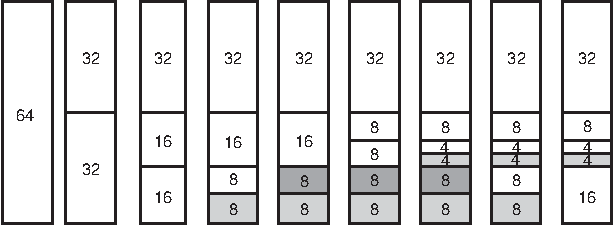
\includegraphics[width=.8\textwidth]{buddy}
    } \mode<article>{
      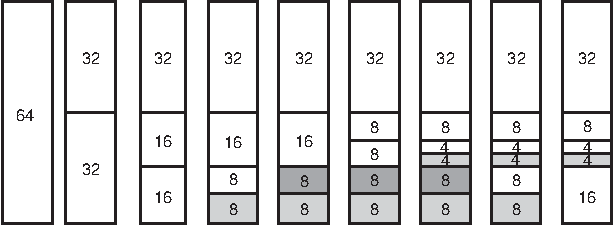
\includegraphics[width=.5\textwidth]{buddy}
    }
  \end{center}
\end{frame}

\begin{frame}
  \begin{exampleblock}{Object creation and deletion}
    \begin{itemize}
    \item are widely employed by the kernel
    \item more expensive than allocating memory to them
    \end{itemize}
  \end{exampleblock}
  \begin{exampleblock}{Slab allocation}
    \begin{itemize}
    \item memory chunks suitable to fit data objects of certain type or size are
      preallocated
      \begin{itemize}
      \item avoid searching for suitable memory space
      \item greatly alleviates memory fragmentation
      \end{itemize}
    \item Destruction of the object does not free up the memory, but only opens a slot
      which is put in the list of free slots by the slab allocator
    \end{itemize}
  \end{exampleblock}
  \begin{exampleblock}{Benefits}
    \begin{itemize}
    \item No memory is wasted due to fragmentation
    \item Memory request can be satisfied quickly
    \end{itemize}
  \end{exampleblock}
\end{frame}

\begin{frame}
  \begin{exampleblock}{Slab allocation}
    \begin{itemize}
    \item[Slab] is made up of several physically contiguous pages
    \item[Cache] consists of one or more slabs.
      \begin{itemize}
      \item A storage for a specific type of object such as semaphores, process
        descriptors, file objects etc.
      \end{itemize}
    \end{itemize}
  \end{exampleblock}
  \begin{center}
    \mode<article>{
      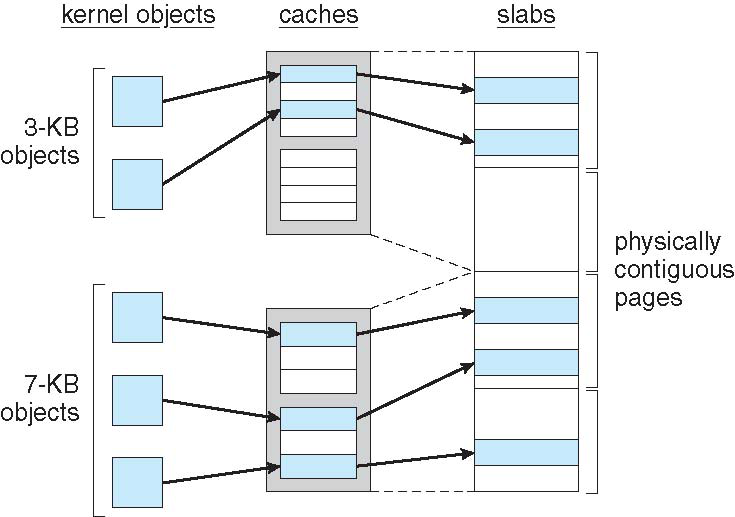
\includegraphics[width=.5\textwidth]{slab}
    } \mode<beamer>{
      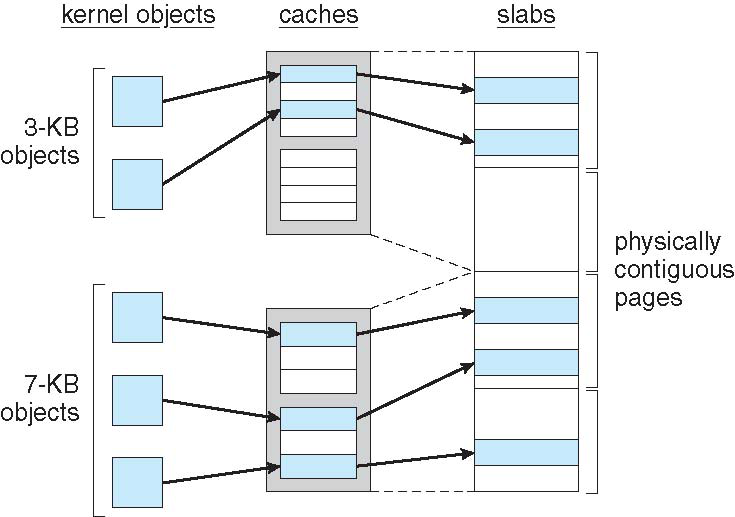
\includegraphics[width=.7\textwidth]{slab}
    }
  \end{center}
\end{frame}

\begin{frame}
  \begin{exampleblock}{Process virtual address space handling}
    \begin{itemize}
    \item demand paging
    \item copy on write
    \end{itemize}
  \end{exampleblock}
\end{frame}

\begin{frame}
  \begin{exampleblock}{Caching}
    \begin{itemize}
    \item hard drives are very slow
    \item to defer writing to disk as long as possible
    \item When a process asks to access a disk, the kernel checks first whether the
      required data are in the cache
    \item \code{sync()}
    \end{itemize}
  \end{exampleblock}
\end{frame}

\subsection{Device Drivers}
\label{sec:device-drivers}

\begin{frame}{Device Drivers}
  The kernel interacts with I/O devices by means of device drivers
  \begin{exampleblock}{The device files in \code{/dev}}
    \begin{itemize}
    \item are the user-visible portion of the device driver interface
    \item each device file refers to a specific device driver
    \end{itemize}
  \end{exampleblock}
\end{frame}

\end{document}

%%% Local Variables: 
%%% mode: latex
%%% TeX-master: "overview-b"
%%% End: 
